 %% Latest change: Thu Mar 11 18:06:33 CET 2010
\documentclass[a4paper]{scrartcl}

\usepackage{ucs}
\usepackage[utf8x]{inputenc}
\usepackage{graphicx}
\usepackage{listings}
\lstset{breaklines=true}
\usepackage{thmbox}
\let\proof\relax
\let\endproof\relax
\usepackage{amsthm}
\usepackage{float}
\setcounter{tocdepth}{2}

\theoremstyle{definition}
\newtheorem*{Def}{Definition}

\title{Whitepaper: \\Protocol-Based Verification for DCP}
\author{Martin Krammer, Clemens Schiffer\\\{martin.krammer,clemens.schiffer\}@v2c2.at\\
Virtual Vehicle Research GmbH, Graz, Austria}
\date{\today{}, Graz}

\begin{document}

\maketitle

\tableofcontents

\section{Introduction}
\label{sec:introduction}
The \textit{Distributed Co-Simulation Protocol} DCP is a platform and communication medium independent standard for the integration of models or real-time systems into simulation environments.
It was specified in course of the ITEA~3 project ACOSAR.
The DCP is standardized by the Modelica Association\footnote{http://www.modelica.org}, where it is maintained as a Modelica Association Project\footnote{http://www.dcp-standard.org}~(MAP).
It is designed to integrate models or real-time systems into simulation environments.
It enables exchange of simulation related configuration information and data by use of an underlying transport protocol (such as UDP, TCP, or CAN).
At the same time, the DCP supports the integration of tools and real-time systems from different vendors.
The DCP is intended to make simulation based workflows more efficient, and to reduce the integration effort.

More detailed information about the DCP can be found in~\cite{Krammer2018,Krammer2019} and on the DCP website.

\section{Target Audience}
\label{sec:audience}
%This document serves as a basis to introduce protocol-based verification to the DCP.
This document is targeted to anyone who aims at implementing the DCP specification.
The target audience includes, but is not limited to:

\begin{itemize}
	\item Software tool vendors
	\item Test system suppliers
	\item System integrators
	\item Simulation engineers
	\item Professionals and students
\end{itemize}

\section{Software Packages and Relationships}
\label{sec:software}

\subsection{Overview}
Right from the beginning, the DCP was intended as an open-access specification, accompanied by open-source software.
The following software projects emerged out of ITEA~3 ACOSAR, and are currently being maintained by Modelica Association.

\begin{itemize}
	\item DCPLib\footnote{https://github.com/modelica/DCPLib} is an open-source software library written in C++.
It provides the necessary packages to create both, DCP master and slave software components to realize distributed co-simulation.
\item DCPTestGenerator\footnote{https://github.com/modelica/DCPTestGenerator} is an open-source software library written in Java.
It transforms a DCP slave description (DCPX) file, a test procedure template, and a test procedure extension to an XML based test procedure. 
It consists of a graph structure, intended for slave verification.
\item DCPTester\footnote{https://github.com/modelica/DCPTester} is an open-source software library written in C++.
It is intended to consume the generated test procedure of the DCPTestGenerator, mount a DCP slave-under-test, and execute the test procedure.
\end{itemize}

\subsection{Relationships}

The basic idea of protocol-based verification for distributed co-simulation is explained in~\cite{Krammer2020}.
The relationship between the DCPTestGenerator and the DCPTester is shown in Figure~\ref{fig:relationships}.

\begin{figure}[H]
	\centering
		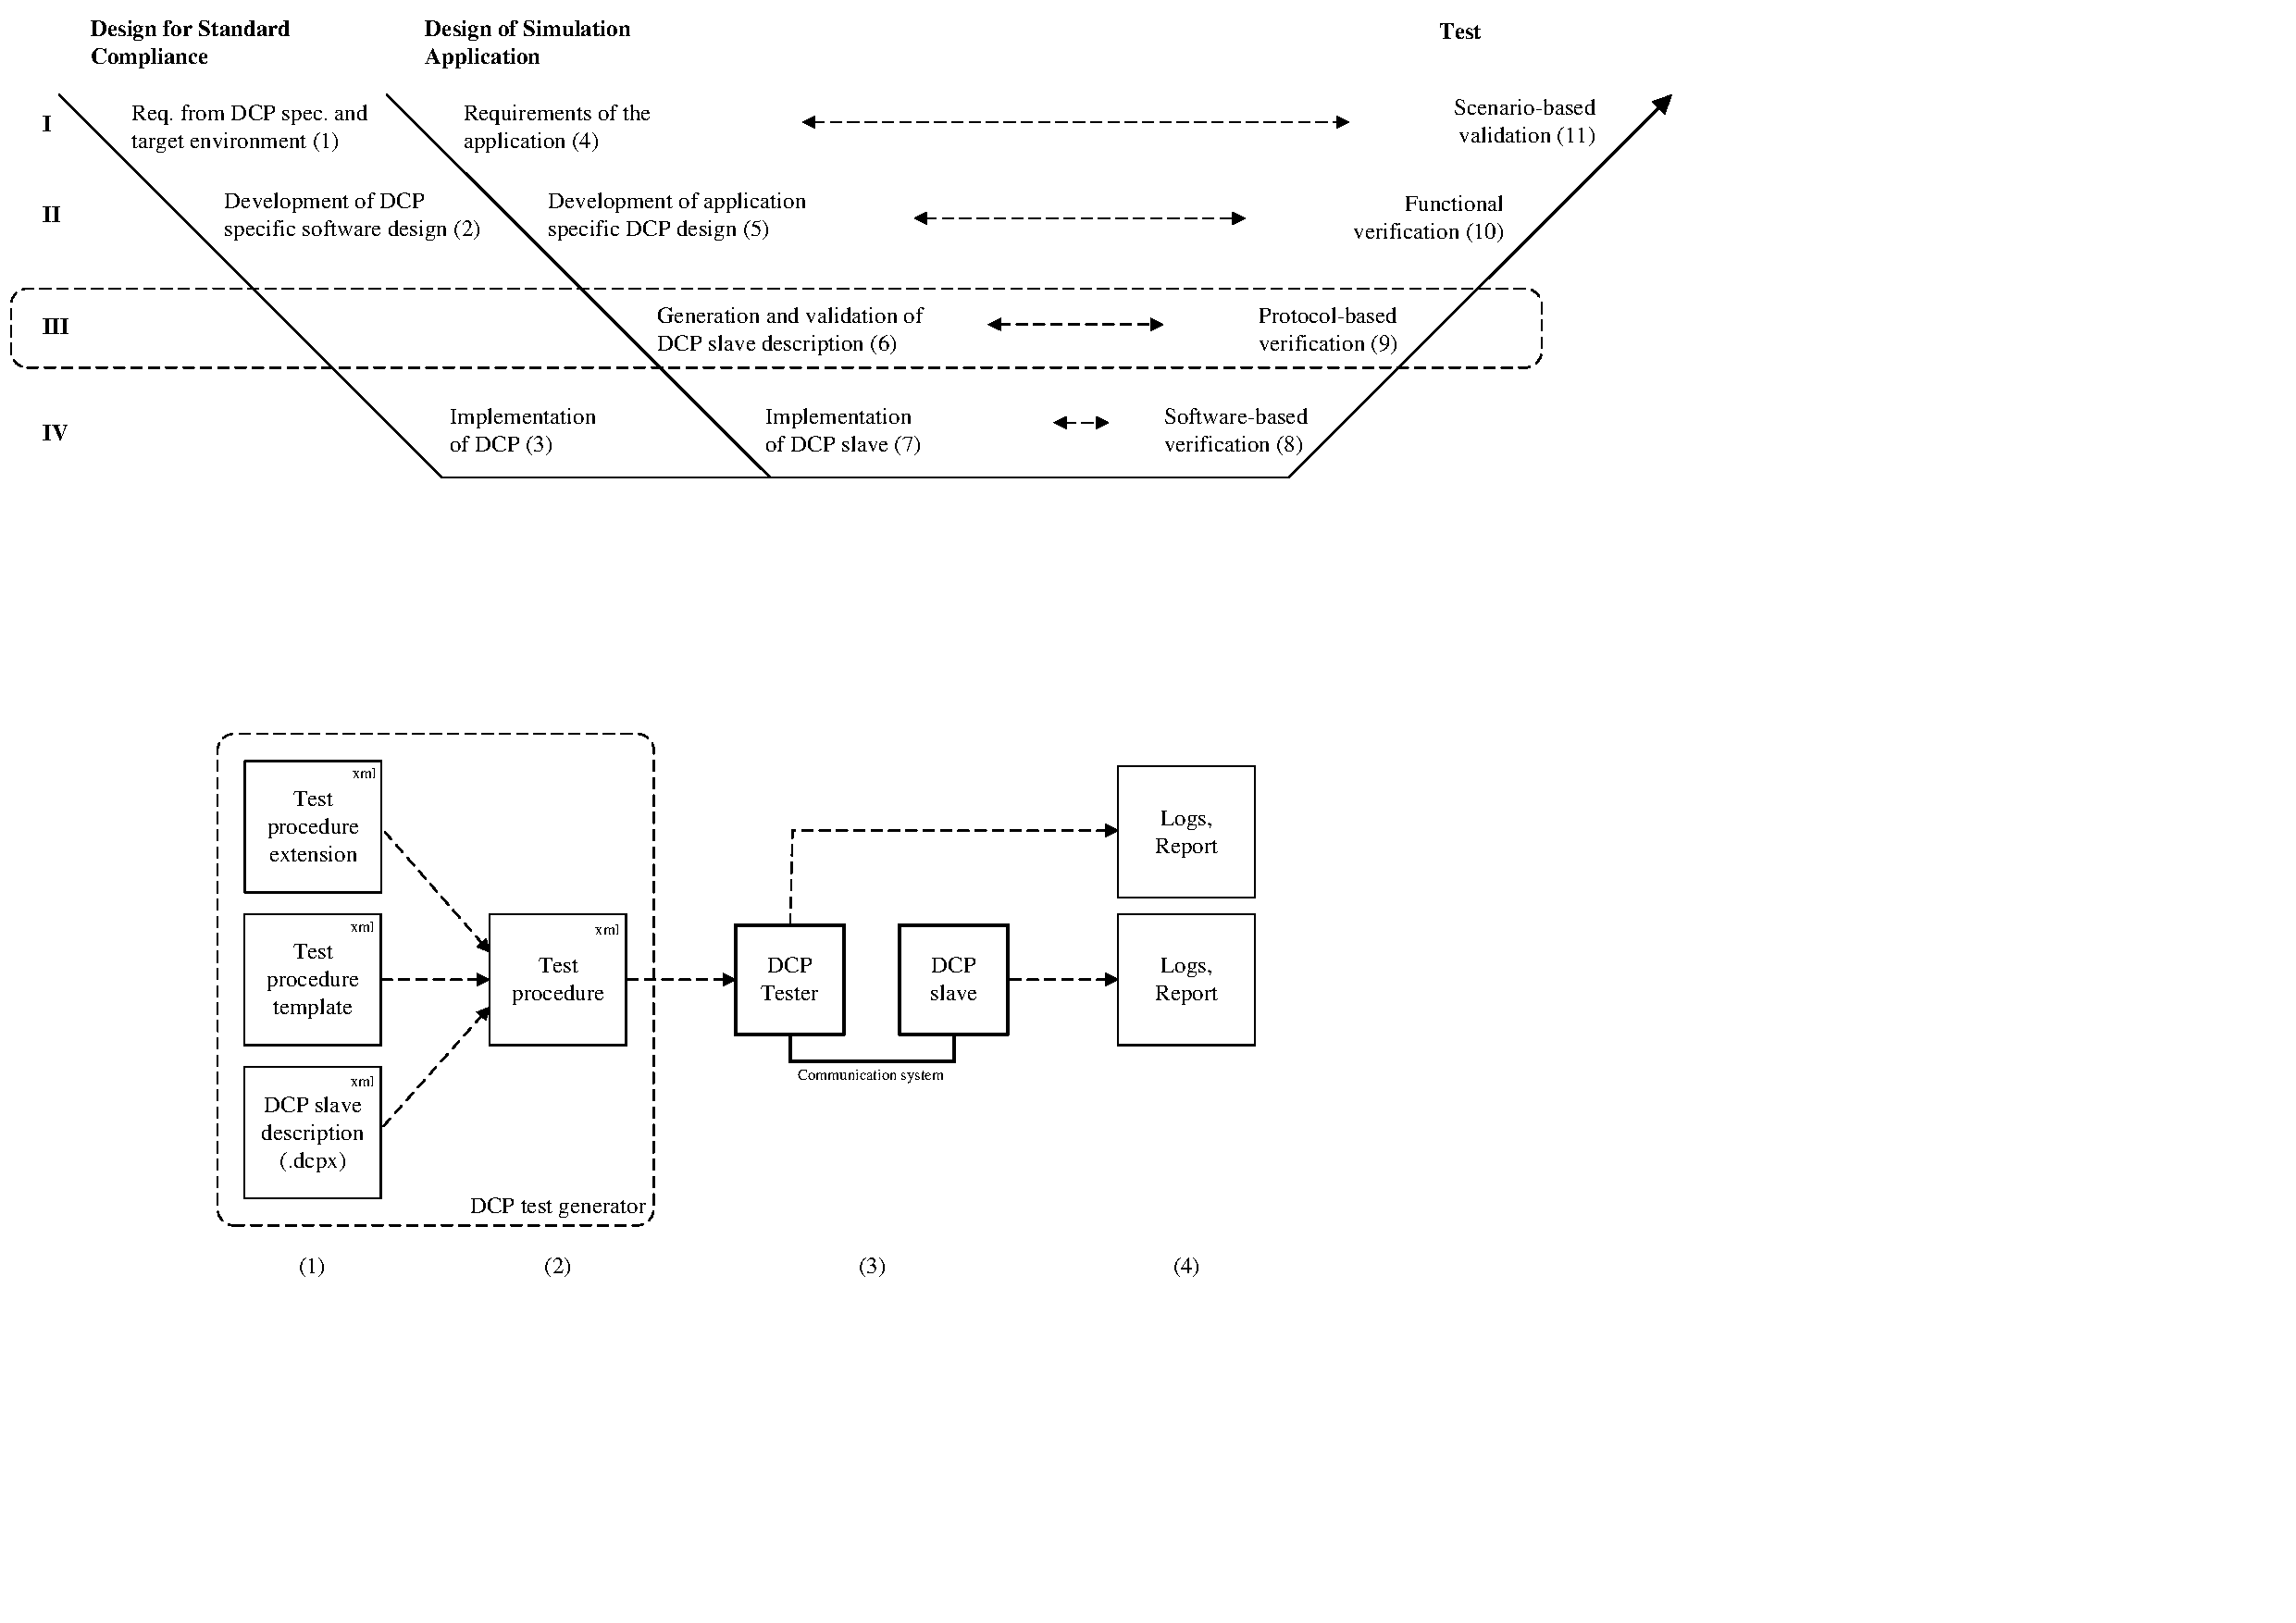
\includegraphics[width=0.95\textwidth, clip=true,trim=3.5cm 6cm 19cm 13cm]{resources/overall_process.pdf}
	\caption{Relationship between DCPTestGenerator and DCPTester~\cite{Krammer2020}.}
	\label{fig:relationships}
\end{figure}

\subsection{Target Version Information}

This document matches the software release numbers provided on GitHub as follows (see Table~\ref{tab:target_version_information}).

\begin{table}[H]
\label{tab:target_version_information}
	\centering
		\begin{tabular}{ll}
			Software	& Version	\\ \hline
			DCPLib	& v0.2 \\
			DcpTester & v0.2 \\
			DcpTestGenerator	& v0.2 \\
		\end{tabular}
		\caption{Software target version numbers.}
\end{table}



\section{Scope and Non-Scope}
\label{sec:scope}
This document is intended as an aid to set up protocol-based testing using the DCP.
Its scope is defined in Figure~\ref{fig:overall_process}.
The dashed line shows the positioning of protocol-based verification in the complete V-diagram.

	\begin{figure}[H]
	\centering % l b r t
 		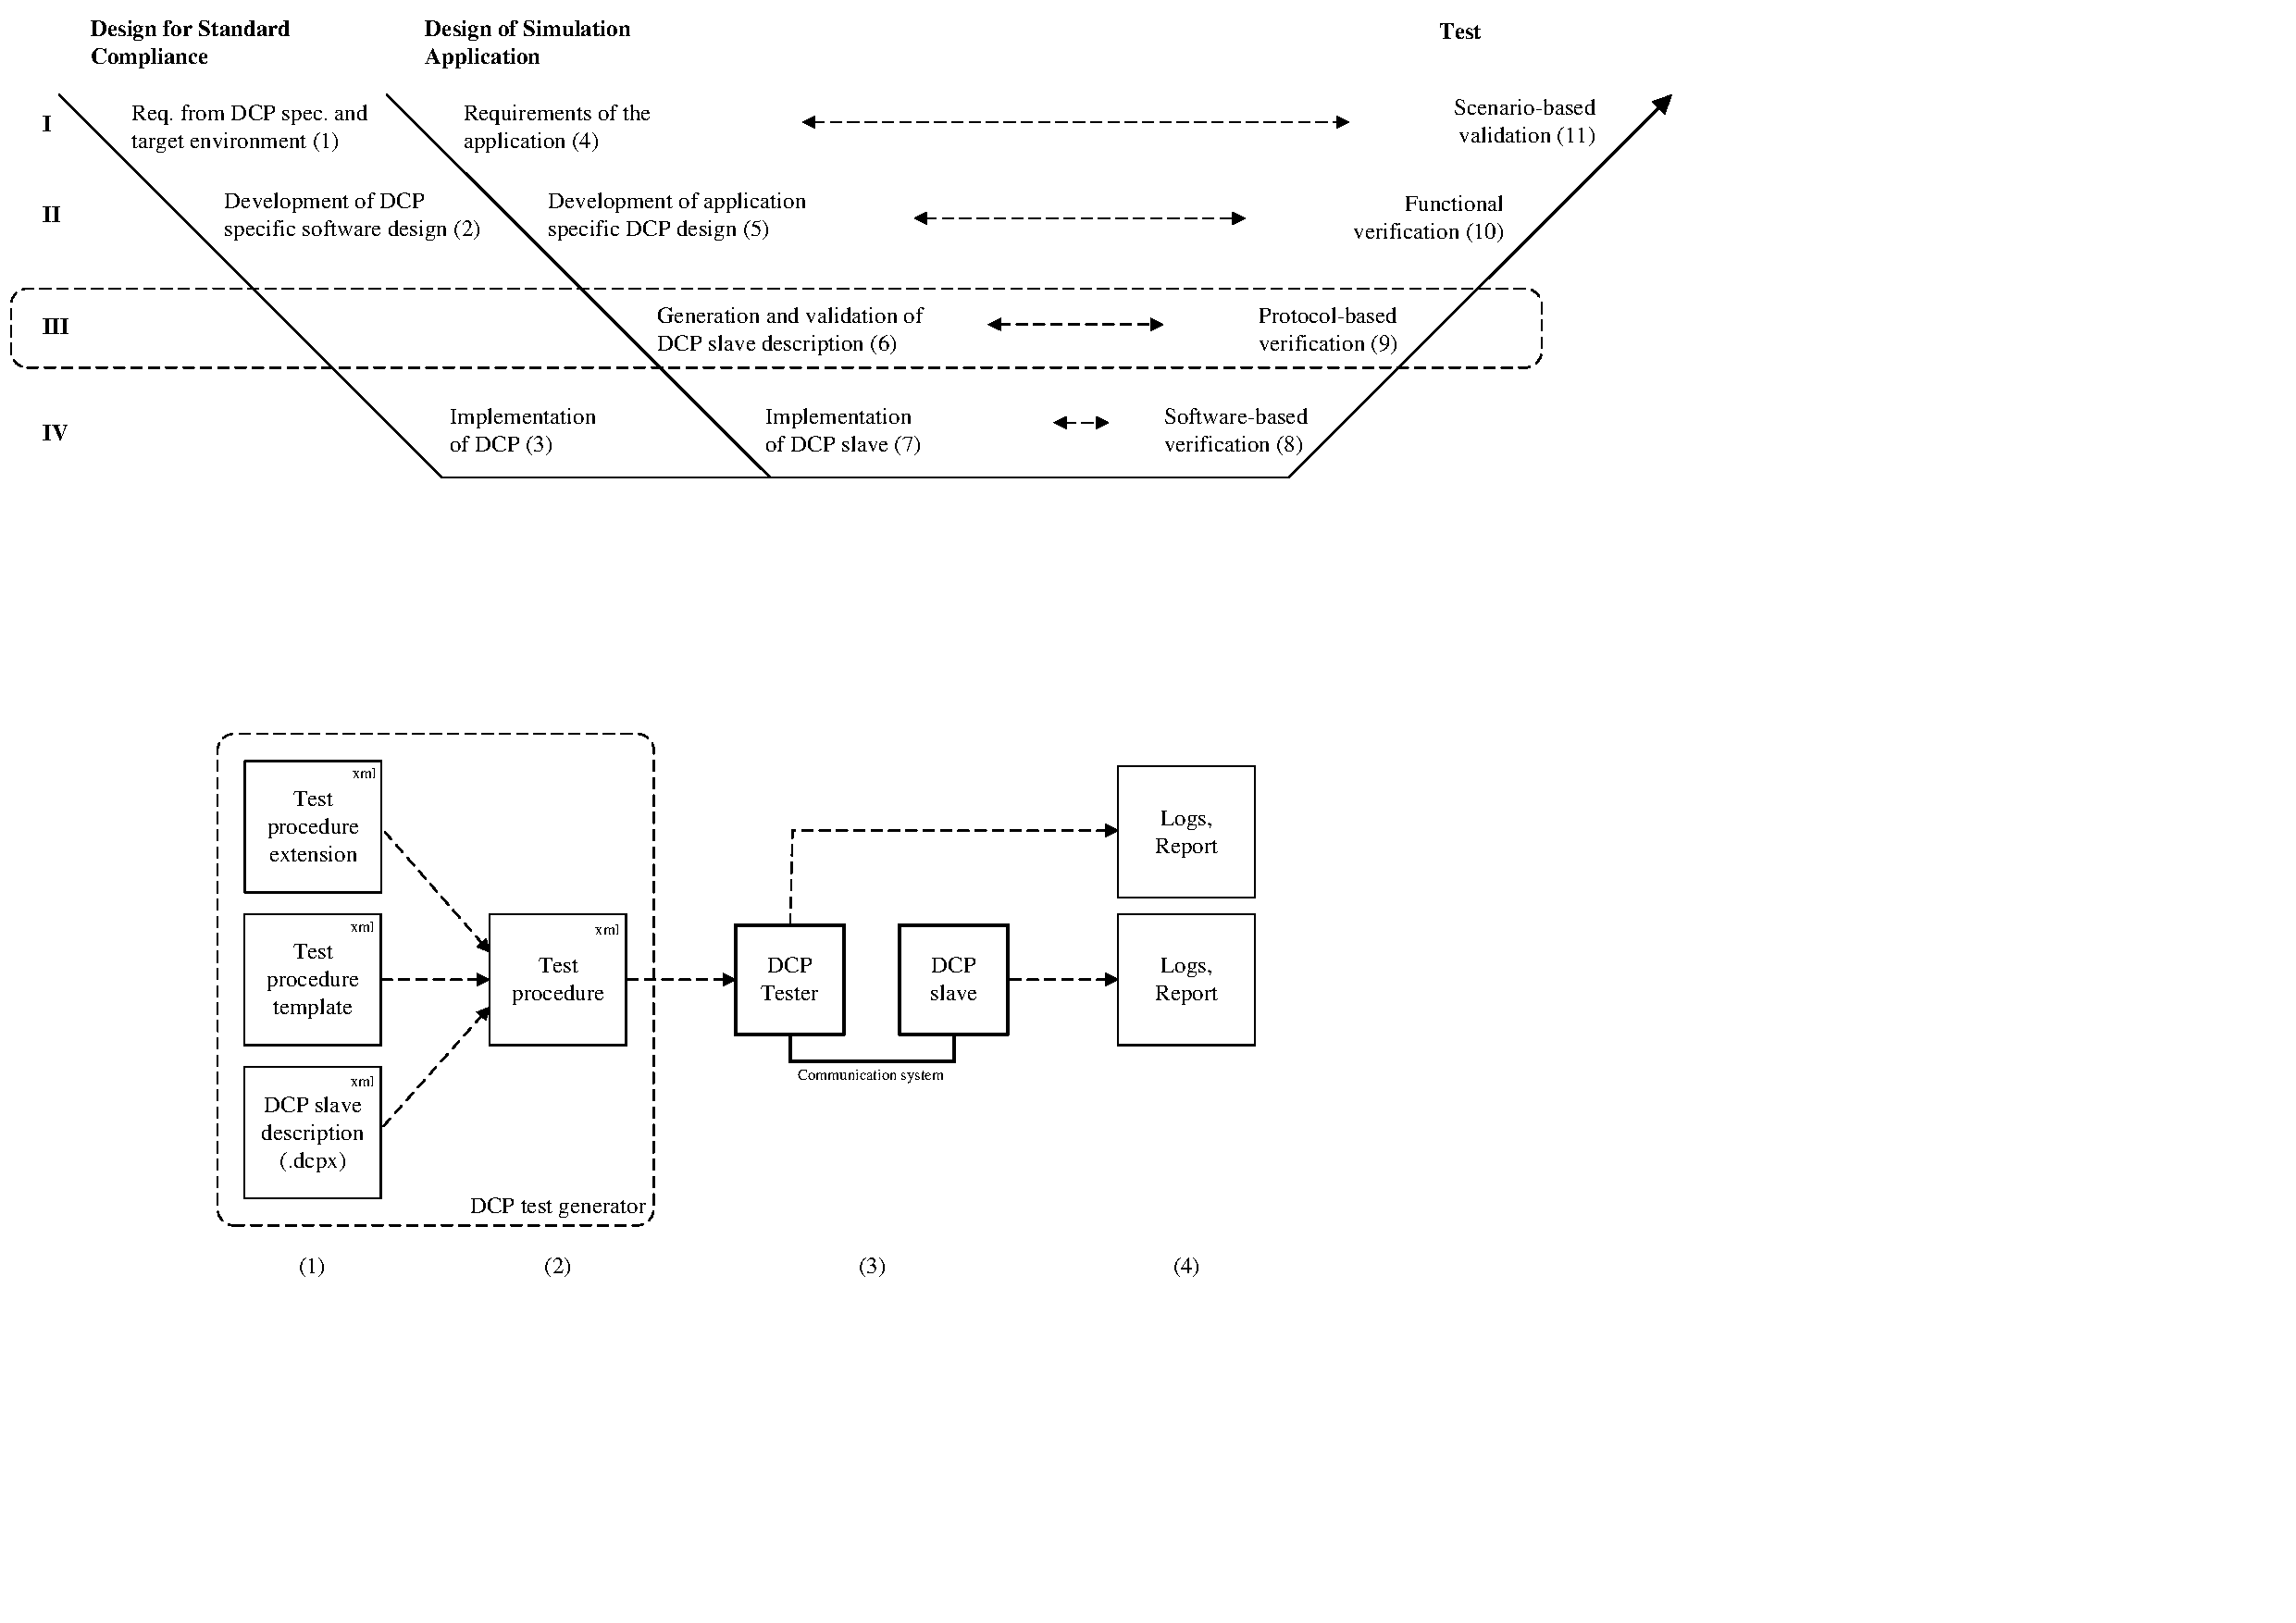
\includegraphics[width=1.0\textwidth, clip=true,trim=0cm 20.5cm 11.5cm 0cm]{resources/overall_process.pdf}
	\caption{V-model for development, verification and validation of a DCP slave~\cite{Krammer2020}.}
	\label{fig:overall_process}
\end{figure}

Its \textbf{non-scope} includes:
\begin{itemize}
	\item Implementation of a slave and associated software-based verification
	\item Application and/or DCP-specific software design and associated functional verification
	\item Scenario-based validation
\end{itemize}

% DCP Test Generator comes with 1 template and 1 extension
% predefined templates
% predefined extension
% kann man nehmen, aber führt zu "`großen"' Test Procedure


\section{DCP Slave-Under-Test}
\label{sec:slave-under-test}
The repository \texttt{DcpTester} provides a DCP slave for demonstration purposes.
It is intended as a sample slave-under-test.
Its DCP slave description (DCPX) file is also provided.
It has the following features:

\begin{itemize}
	\item Support for SRT and NRT operating modes
	\item Support for different resolutions ($5/100$s, $1/10$s, $1/1000$s)
	\item Support for transport protocol UDP IPv4 (TCP also possible)
	\item 12 Input Variables (one for each data type)
	\item 12 Output Variables (one for each data type)
	\item 10 Parameter Variables (one for each data type, excluding binary and string data types)
	\item A basic log category and template
	\item Accepts PDUs from Configuration PDU family (flag set)
	\item Can handle reset (flag set)
	\item Can handle variable steps (flag set)
	\item Can provide log on request (LoR, flag set)
	\item Can provide log on notification (LoN, flag set)
\end{itemize}

The provided DCP slave has no dedicated functionality and assigns the value of an input to the value of an output of the same data type.


\section{Files and Structures}
\label{sec:files_and_structures}

\subsection{Test Procedure Template}
\label{sec:extensions:test_procedure_template}

\subsubsection{Format}
%ToDo: Rename DcpTestProcedure.xsd -> DcpTestProcedureTemplate.xsd
The \textit{Test Procedure Template} can be used for creation of \textit{Test Procedures}.
In fact, it represents a minimum \textit{Test Procedure}, as soon as a UUID of a slave-under-test is added to it, next to connectivity information (Element \texttt{TransportProtocols})

\begin{Def}
The Test Procedure Template is defined by \texttt{DcpTestProcedure.xsd}
\end{Def}

\begin{Def}
\textit{Test Procedure Templates} file names shall comply to the following scheme: \texttt{tpl\_*.xml}
\end{Def}

\subsubsection{Defined Test Procedure Templates}
\label{sec:test_procedure_templates}
The test procedure templates provided are shown in Table~\ref{tab:TestProcedureTemplates}.
These templates are intended for extension by \textit{Test Procedure Extensions}.
This leads to the ability to test DCP slave behaviour in specific states.

Transitions to states that are left via self-triggered transitions (e.g. 4, \texttt{CONFIGURING}) can also be tested, but the slave must remain in this state.
This could require a modification of the implemented slave (e.g. by adding delay), compared to a production slave.

\begin{table}[H]
	\centering
		\begin{tabular}{ll}
		File name & Short Description \\ \hline
		\texttt{tpl\_min.xml}	&	Minimal pass through state machine, no initialization \\
		\texttt{tpl\_stop.xml}	&	Multiple passes through state machine, stop in every state \\
		\texttt{tpl\_to00alive.xml}	& Go to state 0 and stop \\
		\texttt{tpl\_to01configuration.xml} & Go to state 1 and stop \\
		\texttt{tpl\_to03prepared.xml}	& Go to state 3 and stop \\
		\texttt{tpl\_to05configured.xml}	& Go to state 5 and stop \\
		\texttt{tpl\_to07Initialized.xml}	& Go to state 7 and stop \\
		\texttt{tpl\_to10Synchronized.xml}	& Go to state 10 and stop \\
		\texttt{tpl\_to16configured.xml}	& Go to state 16 and stop \\
		\texttt{tpl\_to11configured.xml}	& Go to state 11 and stop, for NRT \\
		\texttt{tpl\_to13configured.xml}	& Go to state 13 and stop, for NRT \\
		\end{tabular}
	\caption{Defined \textit{Test Procedure Templates}}
	\label{tab:TestProcedureTemplates}
\end{table}

\subsection{Test Procedure Extension}
\label{sec:extensions:test_procedure_extension}

\subsubsection{Format}
%ToDo: Rename DCP-Testsuite-extension.xsd \verb+->+ DCPTestProcedureExtension.xsd

\begin{Def}
The \textit{Test Procedure Extensions} are defined by \texttt{DcpTestProcedureExtension.xsd}
\end{Def}

\begin{Def}
\textit{Test Procedure Extensions} file names shall comply to the following scheme: \texttt{ext\_*.xml}
\end{Def}

\subsubsection{Defined Test Procedure Extensions}
List of available extensions

\begin{table}[H]
	\centering
	\footnotesize
		\begin{tabular}{lp{8cm}}
		File name & Short Description \\ \hline
		\texttt{ext\_Min.xml}	&	Add minimal slave specific data \\
		\texttt{ext\_ValidConfiguration.xml} &	Provides a minimal valid configuration (not required when \texttt{canAcceptConfigPdus} set to false) \\
		\texttt{ext\_negativeAllowedPDUsAlive.xml}           & Test rejection of not allowed PDUs in state 0	\\
		\texttt{ext\_negativeAllowedPDUs01Configuration.xml}	& Test rejection of not allowed PDUs in state 1	\\
		\texttt{ext\_negativeAllowedPDUs03Prepared.xml}	& Test rejection of not allowed PDUs in state 3 \\
		\texttt{ext\_negativeAllowedPDUs05Configured.xml}	& Test rejection of not allowed PDUs in state 5	\\
		\texttt{ext\_negativeInvalidConfiguration.xml}   	& Test invalid configuration data	\\
		\texttt{ext\_negativeInvalidValues00Alive.xml}	& Test invalid values in state 0 \\
		\texttt{ext\_negativeInvalidValues01Configuration.xml}	& Test invalid values in state 1 \\
		\texttt{ext\_negativeInvalidValues03Prepared.xml}	& Test invalid values in allowed PDUs \\
		\texttt{ext\_negativeInvalidValues05Configured.xml}	& Test invalid values in allowed PDUs	\\
		\texttt{ext\_negativeInvalidValues07Initialized.xml}	& Test invalid values in allowed PDUs	\\
		\texttt{ext\_negativeInvalidValues10Synchronized.xml}	& Test invalid values in allowed PDUs	\\
		\texttt{ext\_positiveInit.xml}	&	Test initialization loop (100 iterations) \\
		\texttt{ext\_stop.xml}	&	Stop in every state (intended to be used with \texttt{tpl\_stop.xml})	\\ \hline
		\end{tabular}
	\caption{Defined \textit{Test Procedure Extensions}}
	\label{tab:TestProcedureExtensions}
\end{table}


\subsection{Test Procedure }
\label{sec:extensions:test_procedure_extension}

\subsubsection{Format}
%DcpTestProcedure.xsd
If slave specific information is added to the test procedure template, it results in a slave-specific test procedure.

\begin{Def}
The Test Procedure is formally defined by \texttt{DcpTestProcedure.xsd} (same schema file as in~\ref{sec:extensions:test_procedure_template}).
\end{Def}

\begin{Def}
\textit{Test Procedure} file names shall comply to the following scheme: \texttt{proc\_*.xml}
\end{Def}

\subsection{Exhaustive Testing}
\label{sec:exhaustive}
The \textit{DCP Test Generator} was initially released with a set of default templates and extensions.
They were meant for exhaustive testing, as described in~\cite{Krammer2020}.
The delivered files are shown in Table~\ref{tab:TemplatesAndExtensionsForExhaustiveTest}.

\begin{table}[H]
\footnotesize
	\centering
		\begin{tabular}{lp{8cm}}
			File	&	Description	\\ \hline
			\texttt{predefined\_template\_withReset.xml}	&	Covers one pass through the DCP state machine, including the reset transition.\\
			\texttt{predefined\_template\_withoutReset.xml}	&	Covers one pass through the DCP state machine, excluding the reset transition.\\
			\texttt{predefined\_extension\_SRT\_TCP.xml}	&	Extends the templates by steps causing error codes, for TCP transport protocol.\\
			\texttt{predefined\_extension\_SRT\_UDP.xml}	&	Extends the templates by steps causing error codes, for UDP transport protocol.\\ \hline
		\end{tabular}
	\caption{Templates and extensions for exhaustive test.}
	\label{tab:TemplatesAndExtensionsForExhaustiveTest}
\end{table}


\section{How to Create a Custom Template or Extension}
\label{sec:custom}

\subsection{Default Extension Mechanisms}
\label{sec:default_extension_mechanisms}
In this section we want to show an example, how to create a custom template, an extension, and how this results in a new test procedure.
The goal is to send the slave a PDU in state \texttt{CONFIGURATION}  with invalid content and check if the slave reacts with the corresponding error code.
Listing~\ref{lst:example_template} shows an excerpt of a test procedure template.
The template represents the registration procedure of DCP.
After registration the slave transitions to \texttt{CONFIGURATION} state.
In order to do so, the values of \texttt{STC\_register} are generic and need to be replaced with slave specific values.
The template expects to exit the test procedure at step 49 (see at the end of line 2).

\lstset{language=xml, numbers=left, numberstyle=\tiny, numbersep=10pt, frame=lines, captionpos=t, aboveskip=10pt, belowskip=10pt}
\begin{lstlisting}[caption=Snippet of a template, label=lst:example_template]
<?xml version="1.0" encoding="UTF-8" standalone="yes"?>
<DcpTestProcedure version="0.0" name="allPaths.xml" acceptingSteps="49">
    <TransportProtocols/>
    <Transition from="0" to="1">
        <Sending>
            <STC_register receiver="1" state_id="0" op_mode="0"  major_version="0" minor_version="0"/>
        </Sending>
    </Transition>
    <Transition from="1" to="2">
        <Receiving>
            <RSP_ack sender="1"/>
        </Receiving>
    </Transition>
    <Transition from="2" to="4">
        <Receiving>
            <NTF_state_changed sender="1" state_id="1"/>
        </Receiving>
    </Transition>
   ...
\end{lstlisting}

Listing~\ref{lst:example_extension} shows an test procedure extension for the template shown before.
In lines $1-14$ slave specific data from the slave description is used to supplement the template in order to produce a well formed \texttt{STC\_register}-PDU.
This is needed as attributes like, e.g., the \texttt{UUID} represents a slave-specific information, that is not part of the template.
Any transition of the template, which fulfills the given condition, will be updated with corresponding values of the slave description.
The parameter \texttt{state} of \texttt{ExtensionSet} set to $1$ extends all \texttt{CONFIGURATION} states.
It adds several new transitions, with the goal to provoke different error codes in state \texttt{CONFIGURATION}.
The example shows a situation where the tester sends a PDU (\texttt{STC\_prepare}) with a state id of $0$.
Since the slave is in state $1$ (\texttt{CONFIGURATION}), it is specified to reject it with the corresponding error code $8205$.
At the end, \texttt{UpdateMaxStep} is set to $2$, because this branch of the tree data structure is extended by $2$ steps.

\lstset{language=xml, numbers=left, numberstyle=\tiny, numbersep=10pt, frame=lines, captionpos=t, aboveskip=10pt, belowskip=10pt}
\begin{lstlisting}[caption=Snippet of an extension, label=lst:example_extension]
  <ForEach variableName="transition">
    <Set>
      <Test.transitions/>
    </Set>
    <If
      condition="transition.sending!=undefined&amp;&amp;transition.sending.stcRegister!=undefined">
      <Update oldVariable="transition.sending.stcRegister.minorVersion"
        newVariable="slave.dcpMinorVersion"/>
      <Update oldVariable="transition.sending.stcRegister.majorVersion"
        newVariable="slave.dcpMajorVersion"/>
      <Update oldVariable="transition.sending.stcRegister.slaveUuid" newVariable="slave.uuid"/>
      <Update oldVariable="transition.sending.stcRegister.opMode" newVariable="1"/>
    </If>
  </ForEach>

  <ExtensionSet state="1">
    <AddTransition fromOffset="0" toOffset="1">
      <Sending>
        <STC_prepare>
          <Receiver>
            <Value value="1"/>
          </Receiver>
          <StateId>
            <Value value="0"/>
          </StateId>
        </STC_prepare>
      </Sending>
    </AddTransition>
    <AddTransition fromOffset="1" toOffset="2">
      <Receiving>
        <RSP_nack>
          <Sender>
            <Value value="1"/>
          </Sender>
          <ErrorCode>
            <Value value="8205"/>   <!-- INVALID_STATE_ID -->
          </ErrorCode>
        </RSP_nack>
      </Receiving>
    </AddTransition>
    <UpdateMaxStep increase="2"/>
    ...
\end{lstlisting}

Listing~\ref{lst:example_procedure} shows the resulting test procedure.
Note the filled in slave specific data in  \texttt{STC\_register} in  line $3$.
This is followed by permissible state transitions.
In lines $15-19$, however, a  \texttt{STC\_prepare} is sent to the slave-under-test, requesting a correct state, but stating an incorrect current state in the attribute \texttt{state\_id}.
If responding correctly, the slave-under-test should reply using error code $8205$.

\lstset{language=xml, numbers=left, numberstyle=\tiny, numbersep=10pt, frame=lines, captionpos=t, aboveskip=10pt, belowskip=10pt}
\begin{lstlisting}[caption=Snippet of the finished procedure, label=lst:example_procedure]
    <Transition from="0" to="7">
        <Sending>
            <STC_register receiver="1" state_id="0" slave_uuid="0d7217ea-ac72-11ea-bb37-0242ac130002" op_mode="1" major_version="1" minor_version="0"/>
        </Sending>
    </Transition>
    <Transition from="7" to="8">
        <Receiving>
            <RSP_ack sender="1"/>
        </Receiving>
    </Transition>
    <Transition from="8" to="36">
        <Receiving>
            <NTF_state_changed sender="1" state_id="1"/>
        </Receiving>
    <Transition from="36" to="58" log="false">
        <Sending>
            <STC_prepare receiver="1" state_id="0" />
        </Sending>
    </Transition>
    <Transition from="58" to="59" log="false">
        <Receiving>
            <RSP_nack sender="1" error_code="8205"/>
        </Receiving>
    </Transition>
    ...
\end{lstlisting}

\subsection{Advanced Extension Mechanisms}
\label{sec:advanced_extension_mechanisms}
In Listing~\ref{lst:example_procedure_loop} an alternative extension is shown demonstrating the loop capabilities of extensions.
Rather then checking for one specific value of \texttt{state\_id} (as shown in Section~\ref{sec:default_extension_mechanisms}, it is possible to check for a set of incorrect values.
The \texttt{ForEach} statement iterates over all possible DCP states ($0-18$, line $4$), except for the current state (line $6$).
The slave is expected to provide the correct error code ($8205$) for all of these cases.

With this tool many transitions can be generated at once allowing for effective testing of the protocol.

\lstset{language=xml, numbers=left, numberstyle=\tiny, numbersep=10pt, frame=lines, captionpos=t, aboveskip=10pt, belowskip=10pt}
\begin{lstlisting}[caption=Snipped of extension showing loops., label=lst:example_procedure_loop]
  <ExtensionSet state="1">
    <ForEach variableName="oState">
      <Set>
        <DcpStates/>
      </Set>
     <If condition="state!=oState">
      <AddTransition fromOffset="0" toOffset="1">
        <Sending>
          <STC_prepare>
            <Receiver>
              <Value value="1"/>
            </Receiver>
            <StateId>
              <Variable variablenname="oState"/>
            </StateId>
          </STC_prepare>
        </Sending>
      </AddTransition>
      <AddTransition fromOffset="1" toOffset="2">
        <Receiving>
          <RSP_nack>
            <Sender>
              <Value value="1"/>
            </Sender>
            <ErrorCode>
              <Value value="8205"/>  <!-- INVALID_STATE_ID -->
            </ErrorCode>
          </RSP_nack>
        </Receiving>
      </AddTransition>
      <UpdateMaxStep increase="2"/>
    </If>
    </ForEach>
\end{lstlisting}

It is advantageous to use such a dynamic generation of test procedures, especially when testing the configuration of slaves, e.g., iterating over the set of all inputs, and all possible configurations for these inputs.
Possible sets to iterate are given in Table~\ref{tab:iterableSets}.

\begin{table}[H]
\label{tab:iterableSets}
	\centering
		\begin{tabular}{l}
		\textbf{Iterable set} \\ \hline
			Slave.Outputs \\
			Slave.Inputs \\
			Slave.Parameters \\
			DcpStates \\
			DcpOpModes \\
			DcpTransportProtocols \\
			Test.transitions \\
		\end{tabular}
		\caption{Iterable sets for extensions}
\end{table}

Another mechanism is the definition of ranges, so it is possible to iterate over a range of integers, as shown in Listing~\ref{lst:example_procedure_loop_range}.
Using this technique, we can test the entire remaining range of invalid state identifiers, starting from $19$, up to the highest possible (8-bit integer) number $255$.

\begin{lstlisting}[caption=Snipped of extension showing a loop over a range, label=lst:example_procedure_loop_range]
    ...
    <ForEach variableName="invalidState">
    <Set>
        <IntegerRange min="19" max="255"/>
    </Set>
    <AddTransition fromOffset="0" toOffset="1">
      <Sending>
        <STC_prepare>
          <Receiver>
            <Value value="1"/>
          </Receiver>
          <StateId>
            <Variable variablenname="invalidState"/>
          </StateId>
        </STC_prepare>
      </Sending>
    </AddTransition>
    ...
\end{lstlisting}




\section{Docker Container-based Testing}
\label{sec:docker}

\subsection{Basic Procedure}
\label{sec:basic_procedure}
The docker container builds the \textit{DCP Library}, the \textit{DCP Tester}, the \textit{DCP Test Generator} and the provided slave-under-test.
The usage of a docker container has two advantages:
\begin{enumerate}
\item It provides a platform independent encapsulated environment, in which all software components can be build, under consideration of their dependencies.
\item The test procedures are executed on the slave-under-test.
\item At the same time, it provides documentation of the build process, as the Docker-file describes the environment.
\end{enumerate}
The docker can be build as follows (see Listing~\ref{lst:docker1}).

\lstset{language=bash, numbers=left, numberstyle=\tiny, numbersep=10pt, frame=lines, captionpos=t, aboveskip=10pt, belowskip=10pt}
\begin{lstlisting}[caption=Building the Docker container, label=lst:docker1]
git clone https://github.com/modelica/DCPTester.git
cd DCPTester/tester/docker
docker-compose build
\end{lstlisting}

Once the build is complete the docker can be started in interactive mode as shown in Listing~\ref{lst:docker2}.
\begin{lstlisting}[caption=Building the Docker container, label=lst:docker2]
docker-compose run Test bash
\end{lstlisting}

This results in the following folder hierarchy:
\begin{itemize}
	\item \texttt{/cmake}
	\item \texttt{/src/dcptester}
	\item \texttt{/tester/Extensions}
	\item \texttt{/tester/Templates}
	\item \texttt{/tester/SlaveUnderTest}
\end{itemize}

The folders \texttt{Extensions}, \texttt{Templates}, and \texttt{Procedures} contain the files and structures explained in Section~\ref{sec:files_and_structures}.
The folder \texttt{Scripts} contains 2 shell scripts.

\lstset{language=bash, numbers=left, numberstyle=\tiny, numbersep=10pt, frame=lines, captionpos=t, aboveskip=10pt, belowskip=10pt}
\begin{lstlisting}[caption=Test procedure generation, label=lst:test_procedure_generation]
cd Scripts
./generate_Tests.sh
\end{lstlisting}

Line 2 of Listing~\ref{lst:test_procedure_generation} calls the DcpTestGenerator, consumes extensions, templates, and a DCPX file.
The file \texttt{TestsToGenerate.csv} describes which templates are to be combined with which extensions.
The script iterates over this list and produces a set of test procedures, and writes them to a file (\texttt{ListOfTests.txt}).

After generation, the following directories are generated:
\begin{itemize}
		\item \texttt{/tester/Scripts/Procedures}
		\item \texttt{/docker/Shared}
\end{itemize}

\lstset{language=bash, numbers=left, numberstyle=\tiny, numbersep=10pt, frame=lines, captionpos=t, aboveskip=10pt, belowskip=10pt}
\begin{lstlisting}[caption=Test procedure generation, label=lst:run_tests]
./run_list_of_tests.sh
\end{lstlisting}

Listing~\ref{lst:run_tests} executes the slave-under-test and the DcpTester, which consumes the previously generated test procedures.
It produces a set of log files in the folder \texttt{logs}.
After script execution, this folder will hold log files for each test procedure, collected from both the slave-under-test and the tester.
The file names from the tester follow the format \texttt{tester\_proc\_ext\_*.log}.
The file names from the slave-under-test follow the format \texttt{slave\_proc\_ext\_*.log}.
The file \texttt{summary.log} provides an overview about all executed test procedures.
It provides information about the executed test procedures.

Alternatively, all these steps are carried out by issuing the command shown in Listing~\ref{lst:docker_up} on the Docker host system to start the service.

\lstset{language=bash, numbers=left, numberstyle=\tiny, numbersep=10pt, frame=lines, captionpos=t, aboveskip=10pt, belowskip=10pt}
\begin{lstlisting}[caption=Start Docker container and execute the defined service., label=lst:docker_up]
cd DCPTester/tester/docker
docker-compose up
\end{lstlisting}

\subsection{Important Notice on Test Results}
\label{sec:test_results}
In file \texttt{summary.log} the outcome of each test procedure is shown.
The possible outcomes are as follows.

\paragraph{\texttt{SUCCESS}} The test procedure was executed and execution finished in one of the defined accepting steps.
\paragraph{\texttt{REVIEW}} The test procedure was executed and execution did not end in a defined accepting step. This can have two causes:

\begin{itemize}
	\item The tester experienced a step that is not defined in the procedure. It is important to note that the slave behaviour may still be compliant to the DCP specification. Review of the log files is highly recommended. This situation may occur due to non-deterministic behaviour of, e.g., operating system schedulers, network stack implementations, or other sources.
	\item The tester experienced a step that is not defined in the procedure and violates the DCP specification. Review of the log files is highly recommended, to determine if modifications of the slave-under-test are needed.
\end{itemize}

\bibliographystyle{plain}
\bibliography{literature}

\end{document}

